\section{Visual Aids User Study}\label{visual-aids-user-study}

\begin{figure}[htbp]
\centering
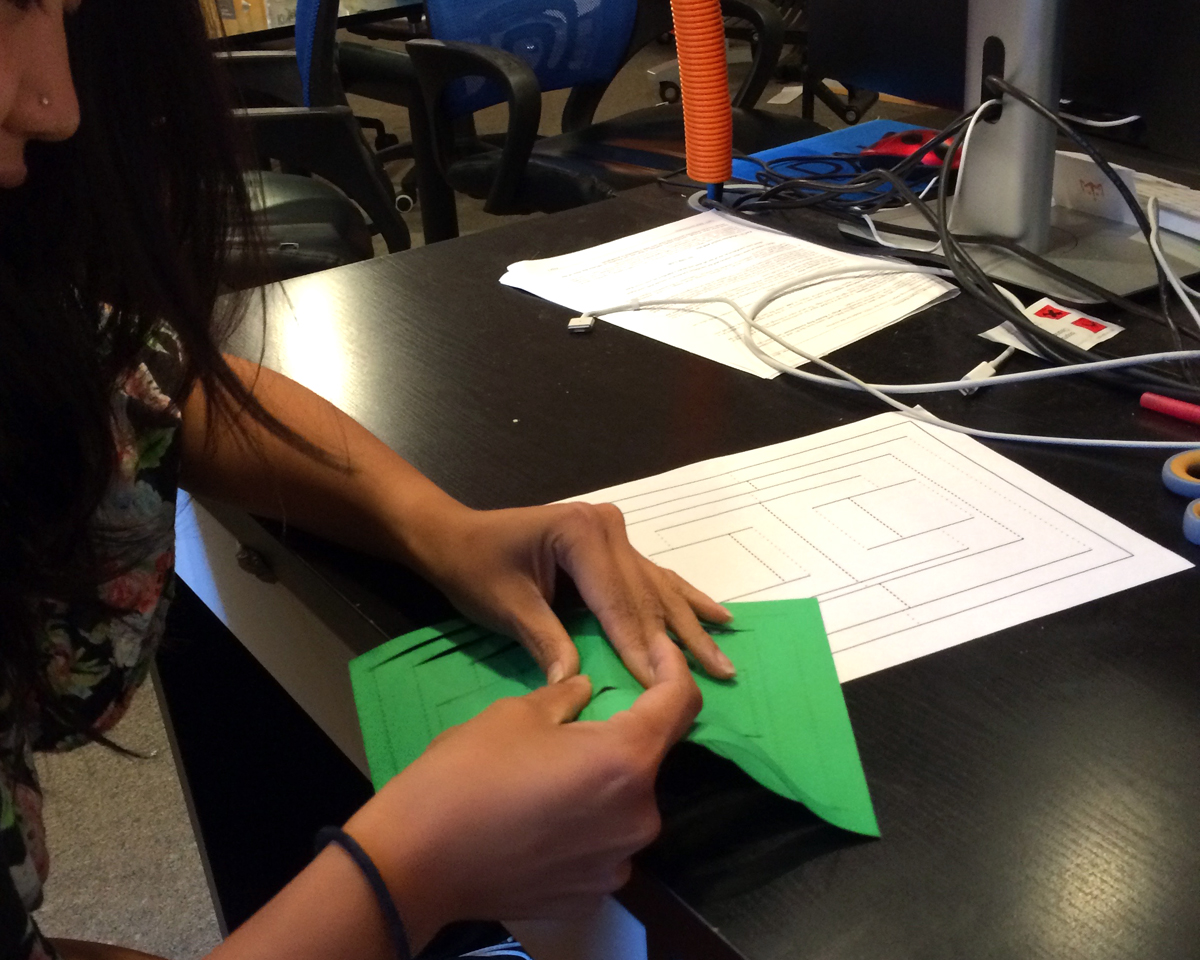
\includegraphics{figures/51_User_Study_Visual_Aids/kikofoldling.jpg}
\caption{A Participant folding a card in our study on 2D to 3D visual
aids for popup cards.}
\end{figure}

The goal of this study was to determine whether users understand the
mapping of 2d fold patterns to 3d, and test the degree to which plane
shading, edge patterning, and a 3d preview help users understand how a
popup card will fold.

\begin{quote}
\begin{quote}
TODO: cite other research on visual aids for folding slash other 2d to
3d vis
\end{quote}
\end{quote}

\subsection{Method}\label{method}

We performed this study with 22 participants, who spent an average of 18
minutes with us. Each subject received a set of five laser cut cards,
and we recorded the time for them to successfully fold the card.
Although there was some variety in age and background, but the largest
demographic was undergraduate Dartmouth students. 10 of the participants
were male, 12 female.

For each card, each subject was randomly given one of of the following
five aids:

\begin{enumerate}
\def\labelenumi{\arabic{enumi})}
\itemsep1pt\parskip0pt\parsep0pt
\item
  A two-dimensional design, showing planes shaded by whether they will
  be horizontal or vertical when folded.
\item
  A two-dimensional design, with edges patterned based on whether they
  are ``hills'' or ``valleys'' --- whether they fold towards or away
  from the card.
\item
  A video showing a simulation of the card folding in three dimensions.
\item
  A still image of the card folded in dimension.
\item
  No visual aid.
\end{enumerate}

The order of aids and cards was shuffled, and then balanced to ensure an
equal distribution of orderings. I.e each visual aid has an equal chance
of being the first aid presented to a user and the last aid presented.

Finally, we asked subjects to rank the visual aids in order of most to
least helpful. For materials used in the study, see Appendix A.

\subsection{Results and Discussion}\label{results-and-discussion}

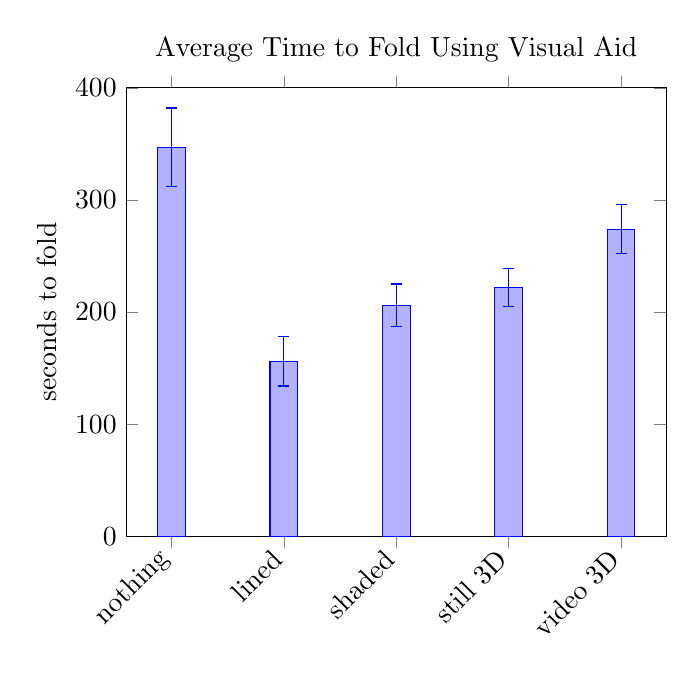
\begin{tikzpicture}
\begin{axis}[
  title=Average Time to Fold Using Visual Aid,
    ybar,
    ymin=0, ymax=400,
    legend style={at={(0.5,-0.2)},
     legend columns=-1},
    ylabel={seconds to fold},
    symbolic x coords={nothing,lined,shaded,still 3D,video 3D},
    xtick=data,
    x tick label style={rotate=45,anchor=east},
]
\addplot+[error bars/.cd,
y dir=both,y explicit]
coordinates {
    (nothing,347) +- (0.0, 35)
    (lined,156) +- (0.0, 22)
    (shaded,206) +- (0.0, 19)
    (still 3D,222) +- (0.0, 17)
    (video 3D,274) +- (0.0, 22)};
\end{axis}
\end{tikzpicture}

The time to fold varied significantly depending on the visual aid used
to fold the card. Error bars indicate a 95\% confidence interval around
the mean, showing a relatively narrow variance within each visual aid
data set. From this, we can conclude that trials with no visual aid were
slower than all trails with visual aids, and that the lined pattern
showing fold orientation was more helpful that any other preview method.
While the shaded visual aid and still 3D preview were indistinguishable,
video 3D was slightly worse than all other visual aids.

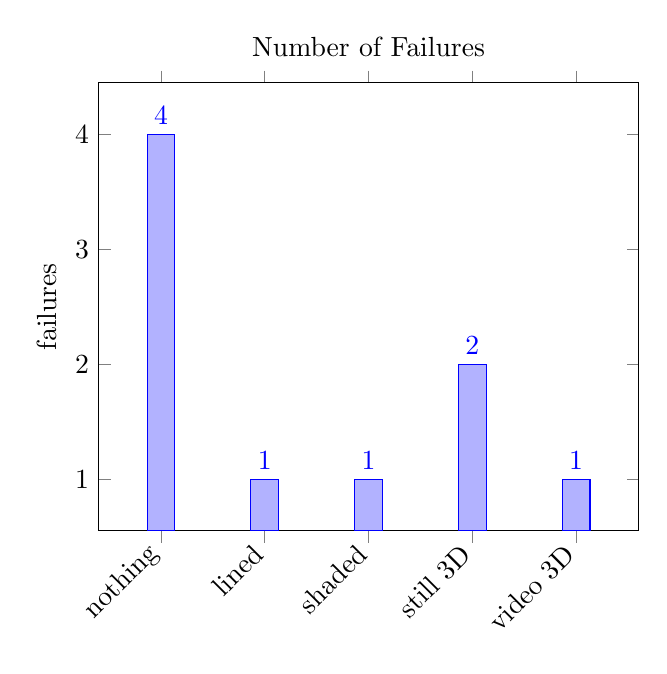
\begin{tikzpicture}
  \begin{axis}[
    title=Number of Failures,
    ybar,
    enlargelimits=0.15,
    legend style={at={(0.5,-0.2)},
      anchor=north,legend columns=-1},
    ylabel={failures},
    symbolic x coords={nothing,lined,shaded,still 3D,video 3D},
    xtick=data,
    nodes near coords, 
    nodes near coords align={vertical},
    x tick label style={rotate=45,anchor=east},
    ]
    \addplot coordinates {(nothing,4)(lined,1)(shaded,1)(still 3D,2)(video 3D,1)};
  \end{axis}
\end{tikzpicture}

Some trials were not completed successfully: either users incorrectly
folded the design. In some cases, they folded the design incorrectly ---
in others, they refused to fold the card, feeling lost without a visual
aid. Unsurprisingly, users were far more likely to fail to fold the card
when they did not have a visual aid. The times for these failures were
not recorded in the Number of Figures graph above.

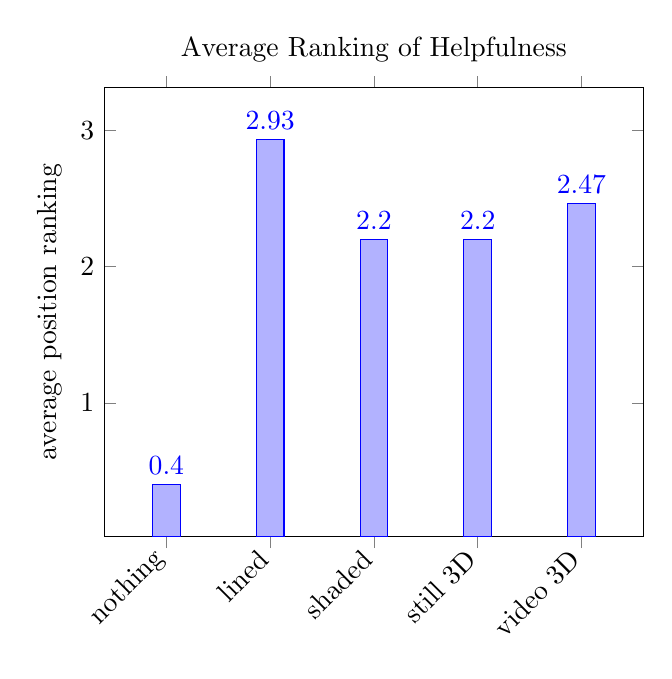
\begin{tikzpicture}
  \begin{axis}[
    title=Average Ranking of Helpfulness,
    ybar,
    enlargelimits=0.15,
    legend style={at={(0.5,-0.2)},
      anchor=north,legend columns=-1},
    ylabel={average position ranking},
    symbolic x coords={nothing,lined,shaded,still 3D,video 3D},
    xtick=data,
    nodes near coords, 
    nodes near coords align={vertical},
    x tick label style={rotate=45,anchor=east},
    ]
    \addplot coordinates {(nothing,0.4)(lined,2.933333333)(shaded,2.2)(still 3D,2.2)(video 3D,2.466666667)};
  \end{axis}
\end{tikzpicture}

We asked subjects to rank the cards from most to least helpful. In this
graph, the data is averaged and inverted (5 being the most helpful), to
show the relatively helpfulness of each aid. Participants rated the
lined aid as the most helpful~---~with small differences among the other
aids, and the lack of visual aid rating very poorly.

While this study gives persuasive evidence for the relative helpfulness
of lines showing fold orientation, it is possible that other aids are
more helpful in completing other 2D to 3D visualization tasks. For
example, it would be interesting to compare the results if we asked
users to simply label horizontal and vertical planes instead of folding
a card. It may be that the lined visual aid was most valuable to this
task because it was closest to the action participants performed: fold
orientation is very closely related to the task of folding a card.

Another limitation of this study is that we fully test the effectiveness
of our interactive 3D preview in helping users visualize the folded
card. We chose to limit the 3D video aid to a non-interactive aid, to
make it more directly comparable to the other visual aids\footnote{If we
  allowed users to interact with the aid, they would have been
  physically split between interacting with the card and interacting
  with the 3D preview. Also, differences in familiarity with iPad use
  might have been a confounding factor if we had used a tablet to
  display the 3D preview}. However, a key benefit of the 3D preview in
our software is that users can directly manipulate and rotate the
simulated card, which was not fully tested in this study.

In Foldlings, we implement many of these visual aids. In the 2D sketch,
we shade planes based on orientation, and display a 3D preview that
users can manipulate in the 3D preview. As a result of our findings in
this study, we also implemented line patterning based on fold
orientation for the SVG export.
